本部分以 Windows 11 系统为例进行安装说明，使用的是常见的 x86\_64 电脑、UEFI 启动和 GPT 分区表。如果你体质特殊,使用的是 Mac，尤其是 Apple Silicon 机型，还请寻找对应的安装方法，不要直接照着下面的分区步骤操作。除此之外，旧式 Legacy/MBR 安装和磁盘加密迁移也需要另外处理。

安装双系统主要分为以下四个流程：系统分区、制作启动盘、从 U 盘进行安装、系统设置相关。下面我们就来一一说明 Ubuntu 22.04 LTS 的安装路线。

\begin{note}
\textbf{动磁盘之前先准备恢复办法。}把你的个人文件备份到另一块介质，并且实际打开几个备份文件确认文件已经备份；保存 Windows 的 BitLocker设备加密恢复密钥，记录磁盘编号、容量与现有 EFI 分区。启动 U 盘中的镜像写入会清空 U 盘；安装器里的格式化会清空选中的分区。看不清是哪块盘时先停下来核对，不按容量猜一个就点确认。
\end{note}

下面四部分连起来，就是一次完整的双系统安装示例。我们先把备份做好，再跟着步骤操作；每一步也会说明做完后应该看到什么，免得点完按钮却不知道到底成功了没有。担心的话，可以照着随堂练习先做记录和判断，确认自己的方案后再真正写盘。

\subsubsection{系统分区}
\label{sec:ubuntu-partition}
制作双系统的第一步，是给 Ubuntu 腾出一块空闲的磁盘空间，这一步我们一般在 Windows 下完成。如果你本来就有未分配空间，可以跳过压缩卷的操作；如果想把原来的整个 D 盘拿来装 Ubuntu，则需要先把里面的文件备份好，因为后面的格式化会清空它。还有一点要注意：Ubuntu 安装器里不会写着“D 盘”，我们要靠磁盘型号、容量和分区布局一起确认。

首先右键桌面上的“此电脑”图标，点击“管理”，进入“磁盘管理”界面。在这里你一般会看到电脑上的若干个磁盘分区，如下图所示。对照磁盘编号与容量，找到准备腾空间的普通数据卷，EFI、恢复和厂商保留分区先不要动。
\begin{figure}[H]
\centering
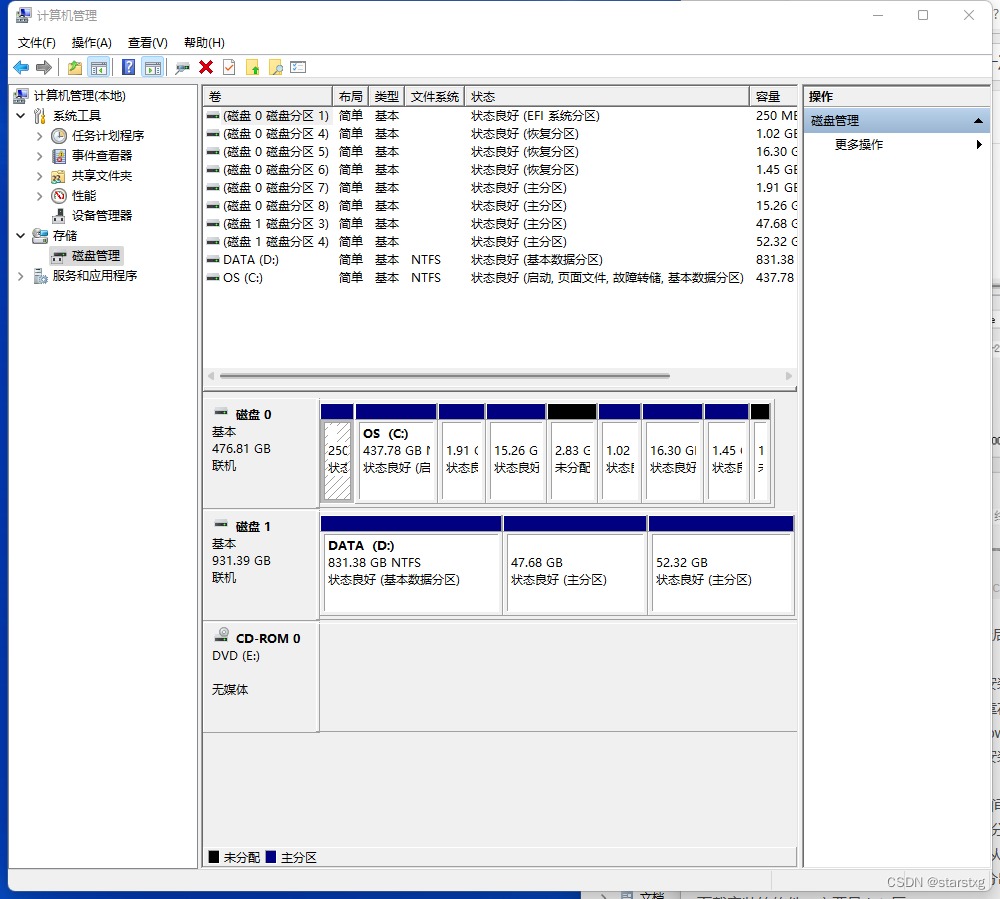
\includegraphics[width=0.75\textwidth]{linux1.png}
\caption{Windows 磁盘管理界面}
\label{fig:linux1}
\end{figure}
接下来选择一个剩余空间较大的普通数据卷，右击，点击“压缩卷”，等待计算完成后，界面会显示当前可用的压缩空间大小。输入你要留给 Ubuntu 的空间量，注意这里的单位标为 MB，规划时可以按约 $1024$ MB 对应 $1$ GiB 换算。图中的 $102400$ 约为 $100$ GiB，只是这台电脑的选择，不用照抄。课程代码本身占用不大，但后面的图像数据集，项目工程以及各类环境会很快长大，有条件可以预留约 $200$ GiB，后续空间不够虽然可以扩容，操作起来却有点麻烦。当然，也别为了凑这个数把 Windows 挤得没地方用了。
\begin{figure}[H]
\centering
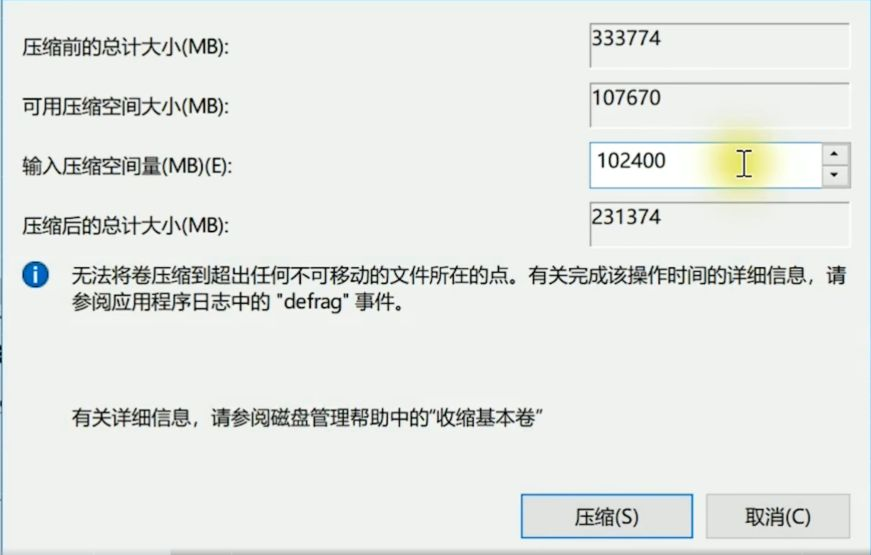
\includegraphics[width=0.75\textwidth]{linux2.jpg}
\caption{压缩卷：读取可压缩空间，再填入自己的容量}
\label{fig:linux2}
\end{figure}
输入好后点击“压缩”，压缩完成后出现一个“未分配”的区域，就说明这一步完成了。\textbf{把它留在未分配状态，不要在 Windows 中新建卷或格式化}，我们等会儿交给 Ubuntu 安装器来处理。如果压缩不到预期大小，先记录界面的限制和现有布局，不要随手删除旁边的分区来凑空间。
\begin{exercise}\label{ex:v1-partition-plan}
记录本机启动模式、分区表类型、各分区容量及剩余空间，规划 Ubuntu 的挂载点与容量。指出已有 ESP 和绝不能格式化的 Windows 分区。
\end{exercise}

\subsubsection{制作启动盘}
首先需要一只容量至少 16 GB 的 U 盘，请先对其中的文件进行备份，后续写入镜像会清空这个 U 盘。

然后进入 Ubuntu 官网下载镜像，下载链接为 \url{https://releases.ubuntu.com/22.04/}。本节截图对应 22.04.5，注意选择 Desktop amd64 的 ISO 文件，不要误下成服务器版。下载好后，我们再按同页的 SHA256SUMS 核对一下文件，具体方法可以看\href{https://ubuntu.com/tutorials/how-to-verify-ubuntu}{Ubuntu 官方镜像校验教程}。ISO 是\textbf{镜像文件}，不是解压后把里面的文件复制到 U 盘就能启动的普通压缩包，所以可别傻傻的直接解压复制。

镜像下载好后，还需要一个启动盘制作器把它写入 U 盘。这里介绍操作比较直观的 balenaEtcher，你也可以按对应说明使用 Rufus 等其他工具。balenaEtcher 的下载链接为 \url{https://etcher.balena.io/}。

安装后点击“Select image”（新版可能叫“Flash from file”）选择刚刚下载的 Ubuntu 镜像，随后在“Select target”中选择你的 U 盘。\textbf{这时候再核对一次设备名和容量，确认没有选到移动硬盘或其他资料盘}，最后点击“Flash!”。等待写入和校验都完成，再安全弹出 U 盘，这样启动盘就做好了。
\begin{figure}[H]
\centering
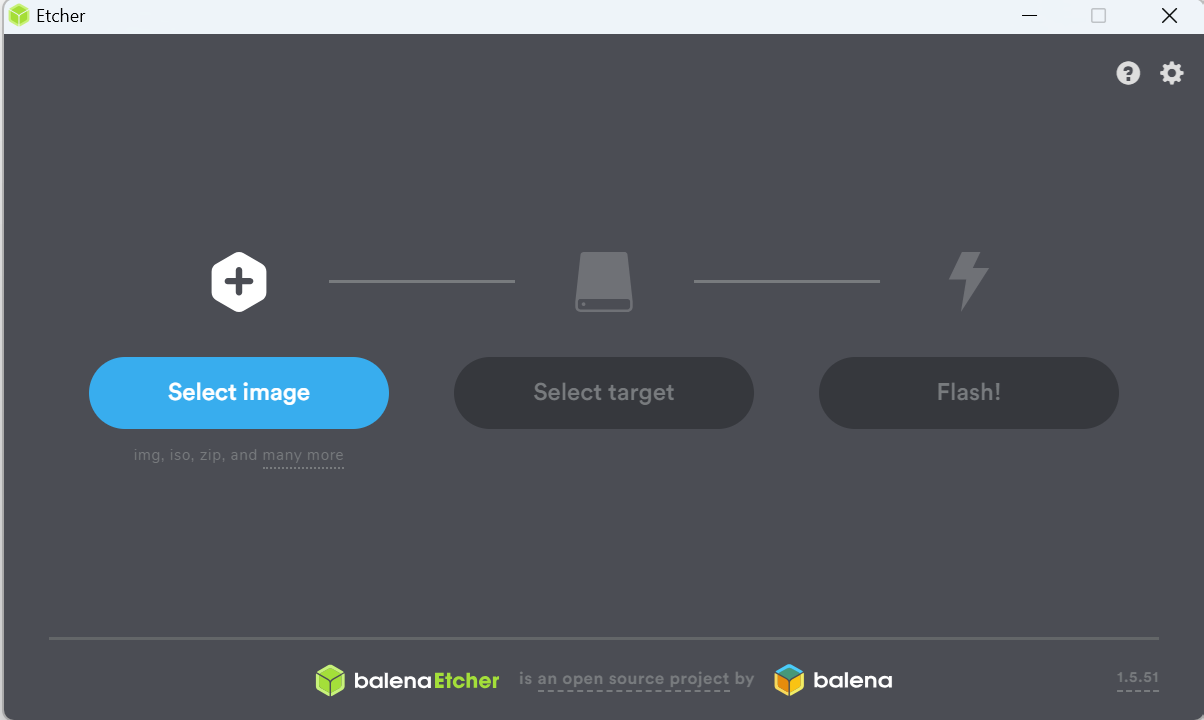
\includegraphics[width=0.8\textwidth]{linux3.png}
\caption{Etcher 界面：镜像、目标盘与写入三个入口}
\label{fig:linux3}
\end{figure}
启动盘做好后，再插到 Windows 中，可能会弹出“需要格式化”的提示。这一般是因为 Windows 不能识别其中所有分区，\textbf{取消提示就好，不要为了消除弹窗把启动盘格式化}，不然你就要重头再来了。这种镜像写入方式也不保证剩余空间还能继续存普通文件，所以资料另找地方放。启动盘被称为“数字生命”，请好好保存，如果后续系统出问题了需要重装，你还用得到它。
\begin{exercise}\label{ex:v1-usb-image}
核对下载的 ISO 校验值，记录 Etcher 中的镜像名称、目标容量及写入校验结果。
\end{exercise}

\subsubsection{从 U 盘进行安装}
插入之前做好的启动盘，接下来我们要让电脑从它启动。在 Windows 中可以按住 Shift 点击“重启”，然后进入“疑难解答”→“高级选项”→“UEFI 固件设置”；也可以重启时按电脑手册里写的快捷键，进入一次性启动菜单。各个主板的按键不太一样，先查清楚再按，否则你可能得“脸滚键盘”了。

\begin{figure}[H]
\centering
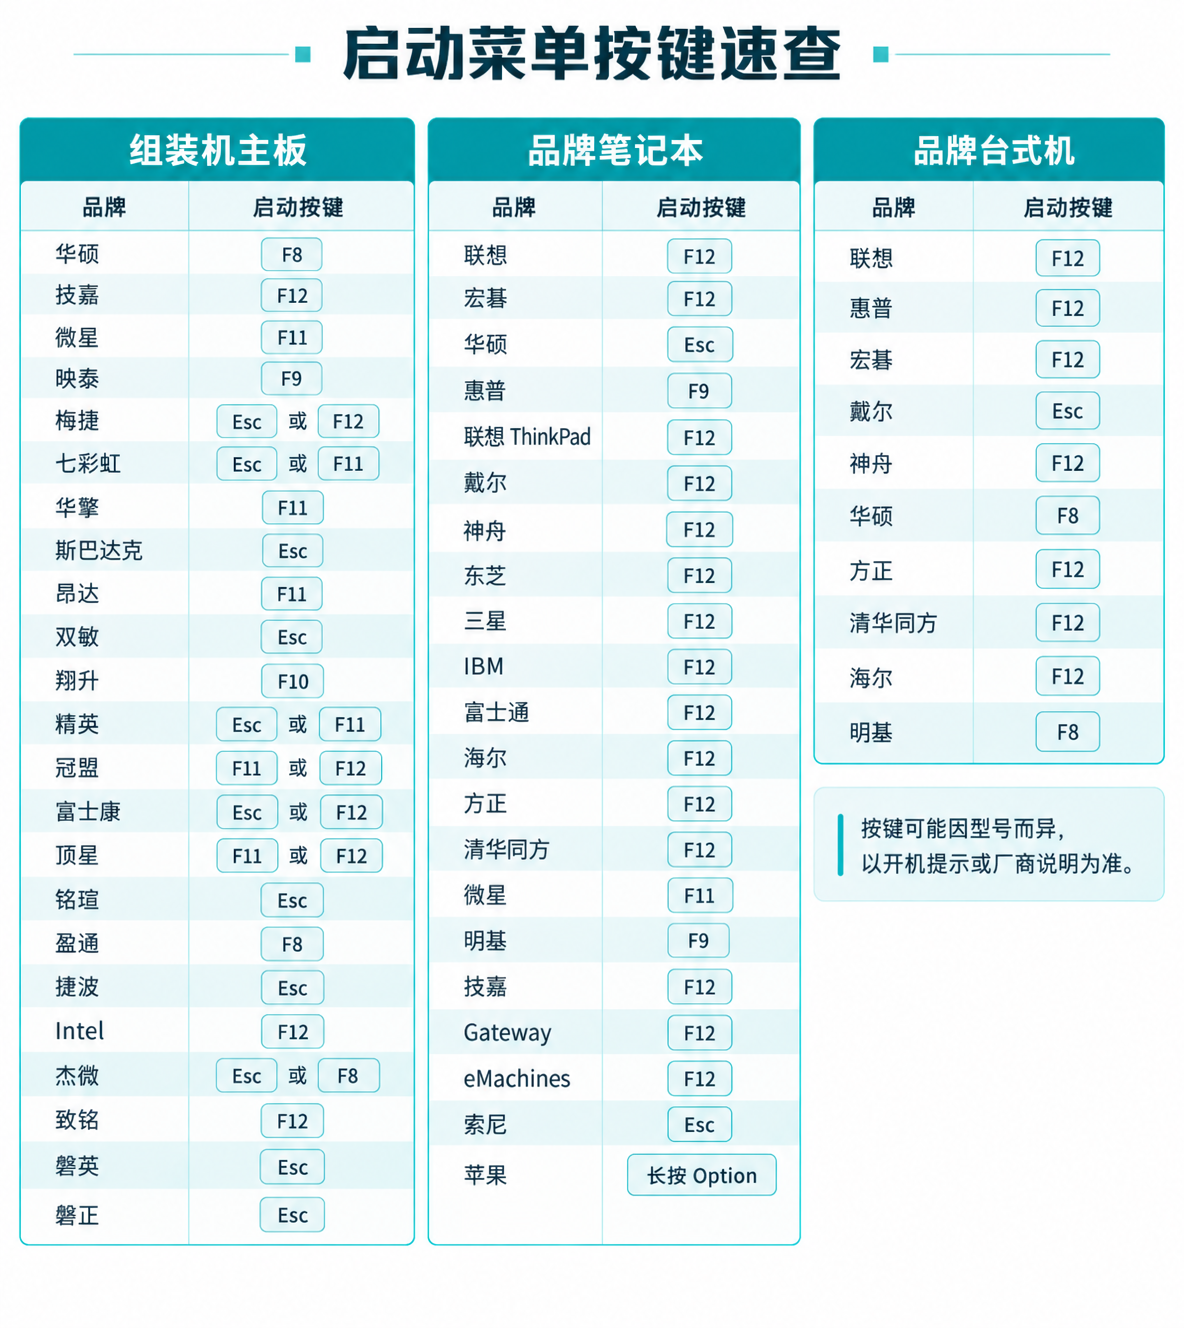
\includegraphics[width=0.8\textwidth]{install1_revised.png}
\caption{启动菜单按键速查}
\label{fig:install1}
\end{figure}

进入启动选项界面后，选择这只 U 盘对应的 UEFI启动项，回车。它可能显示为 Linpus lite，也可能是 Kingston、SanDisk 等品牌名，认准自己的 U 盘即可，不必纠结名字是否和截图一致。接着选择 Install Ubuntu，开始正式安装。

\begin{figure}[H]
\centering
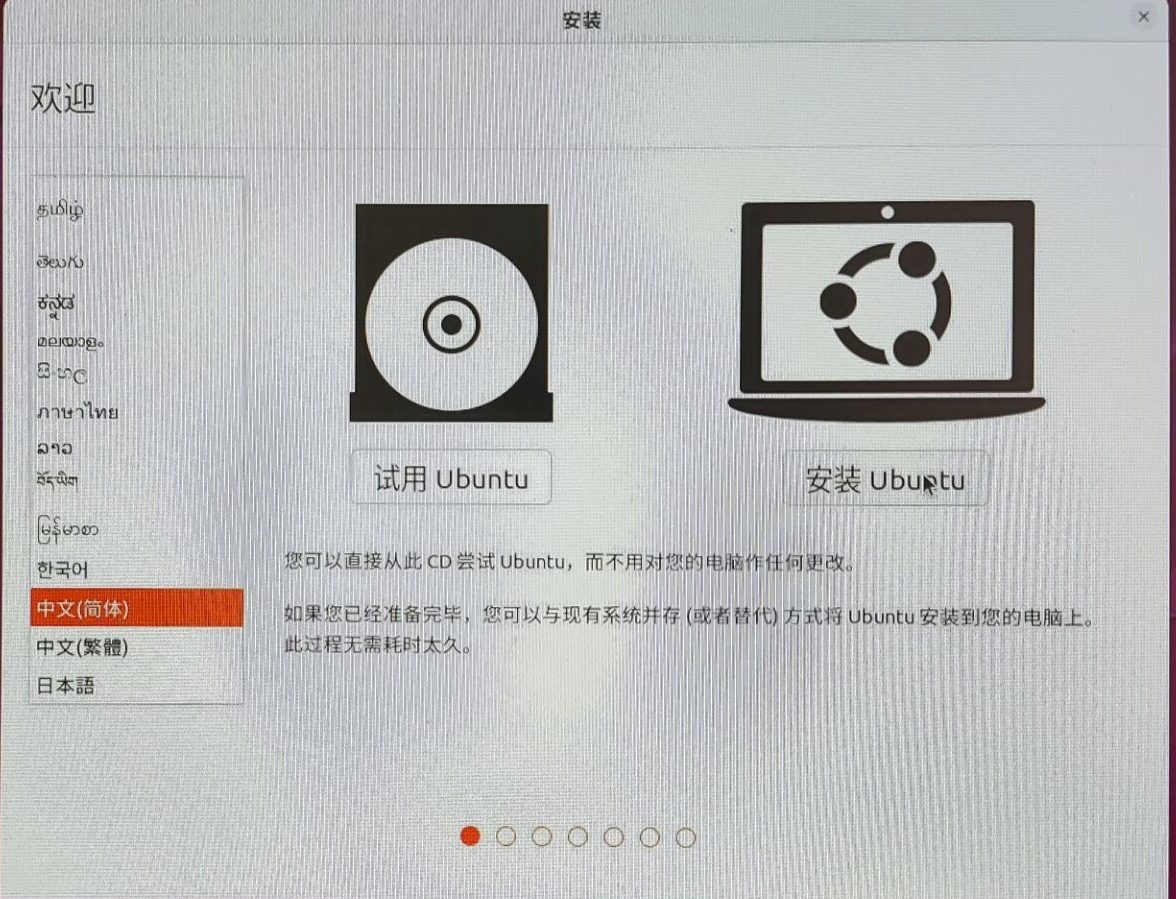
\includegraphics[width=0.75\textwidth]{install2.jpg}
\caption{安装 Ubuntu}
\label{fig:install2}
\end{figure}

首先选择语言为简体中文，“键盘布局”按你实际使用的键盘选择，无线连接和更新可以按当前网络条件决定。然后在“更新和其他软件”页面选择“正常安装”，按硬件需要勾选第三方驱动。
\begin{figure}[H]
\centering
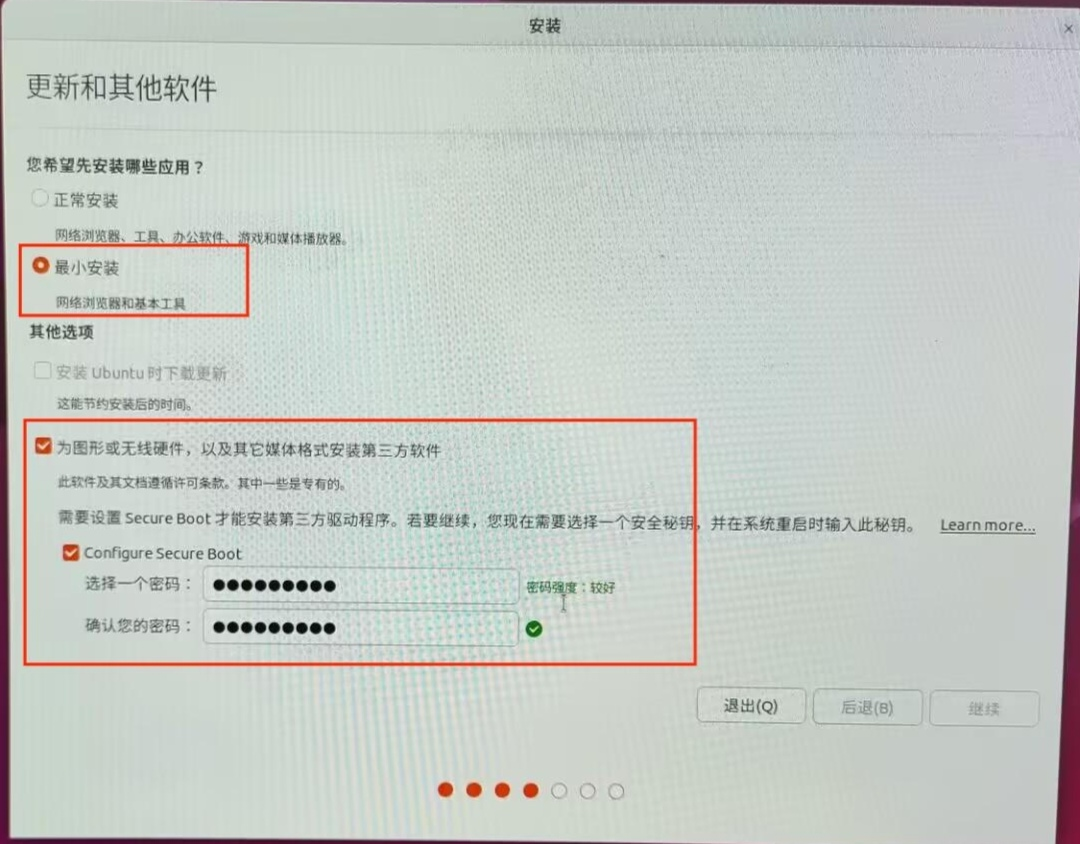
\includegraphics[width=0.75\textwidth]{install3.jpg}
\caption{第三方驱动与 Secure Boot 设置}
\label{fig:install3}
\end{figure}
如果启用了 Secure Boot，安装第三方驱动时可能要求你设置 MOK（Machine Owner Key，机器所有者密钥）注册密码。这个密码是给重启后的密钥注册用的，记下来，到时候按提示确认即可。它不是 Ubuntu 账户的登录密码，后面我们还要另外建立账户，别看到这里填过密码就把后面的步骤跳过去了。

接下来来到“安装类型”，本教程选择\textbf{“其它选项”}，这样我们可以按照刚才的规划手动分区，也能看清究竟要格式化哪些地方。有的安装器会提供“与 Windows 共存”的自动方案，你可以按实际情况选择，但最后的写盘摘要一样要核对。这里最需要注意的是：\textbf{千万不能选择抹掉整个磁盘}，否则留下来的就不是双系统了，到时候只能对着消失的Windows哭泣，重装整个Windows系统。
\begin{figure}[H]
\centering
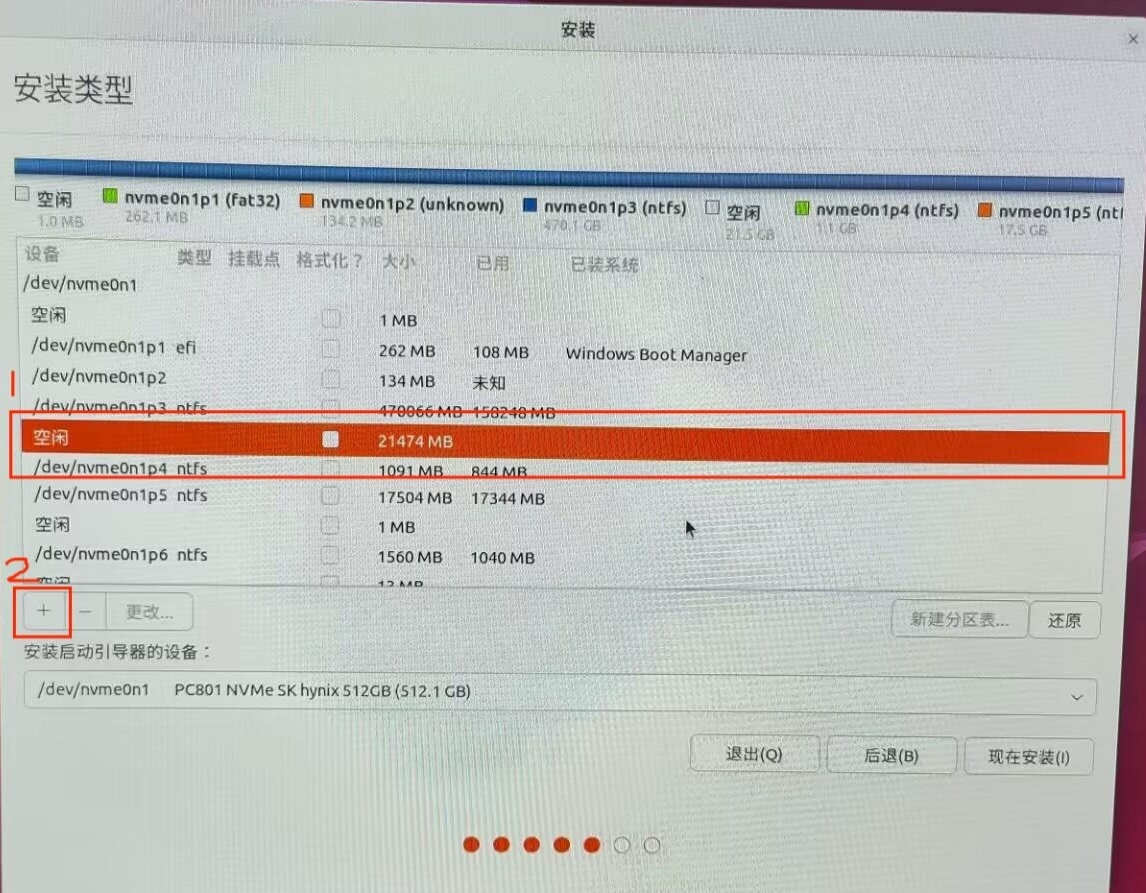
\includegraphics[width=0.8\textwidth]{install4.jpg}
\caption{手动分区：找到之前腾出的空闲空间，图中的设备编号不能照抄}
\label{fig:install4}
\end{figure}
首先找到电脑已有的 EFI 系统分区（EFI System Partition，ESP），它通常是 FAT32，里面有 Windows Boot Manager。我们复用它作为 \texttt{/boot/efi}，\textbf{不要勾选格式化}，Windows 也要靠它启动。这里的 ESP 和存放 Linux 内核的 \texttt{/boot} 不是同一个东西，名字看起来相近，却不能互相替代。如果你的电脑有多块硬盘，需要选择你安装 Ubuntu 的那块硬盘上的 ESP。

然后找到之前压缩出来的空闲区域，点击加号，在这里创建 Ubuntu 的 ext4 分区。你可以按下面两种思路来安排：
\begin{itemize}
\item \textbf{全部放在根分区里。}只创建一个挂载到 \texttt{/} 的分区，用户文件也就放在这个分区里的 \texttt{/home} 目录。这种方式最简洁，适合先把系统用起来；不过日后格式化根分区时，个人文件也会一起被清空。
\item \textbf{把根分区与个人文件分开。}可以给 \texttt{/} 约 80 GiB，再把剩余空间给独立的 \texttt{/home}。这个容量只是例子，你可以按需求调整。以后重装时可以选择保留 /home，不过仍然要先备份，并在安装器里\textbf{明确取消它的格式化}。
\end{itemize}
普通入门安装一般不需要另建 \texttt{/boot}。交换空间（Swap）则可以用安装器建立的交换文件；如果你选择单独建立交换分区，类型选“交换空间”即可。一般来说可以为其分配约 8或16 GiB，或者按电脑内存大小来定。

如果你看过一些旧教程，可能还记得“先分逻辑分区，再分主分区”的说法。不过本节使用的是 GPT，并不按 MBR 的主分区、逻辑分区来安排，也没有这个先后规则。UEFI 的引导文件写入 ESP，\textbf{不要把某个 /boot 分区当作通用的引导安装目标}。如果电脑有多块硬盘，还要看清安装器究竟选中了哪个 ESP；不确定时请学长一起检查，这里多花几分钟，总比装完再抢救省事。相关说明见 \url{https://help.ubuntu.com/community/UEFI}。

\begin{conclusion}
启动模式、分区表、文件系统、挂载点分别管不同的事：UEFI 是怎样启动，GPT 是怎样记录分区，ext4 是怎样存文件，\texttt{/} 与 \texttt{/home} 是从哪里访问文件。已有 ESP 要保留，是否拆分 /home 只影响管理方式，不能代替备份。
\end{conclusion}
\begin{exercise}\label{ex:v1-installer-review}
在纸面方案中给每个分区标记“保留/格式化”及挂载点，并解释 ESP、/boot、swap 的区别。
\end{exercise}

分区安排好后，先别急着点“现在安装”，我们再看一遍写盘摘要：Windows 数据分区和 ESP 都不应该出现在格式化清单里，要格式化的是这次新建的 Ubuntu 分区。确认没有问题后再继续。分区完成后，安装最难的一步就结束了，下来只需要选择时区、账户名和登录密码，等待系统安装完成就好了。

出现安装完成的提示后点击“现在重启”，等到屏幕提示“Please remove the installation medium, then press ENTER”时，拔掉启动盘并按回车。先试着进入 Ubuntu，再重启一次确认 Windows 也能进入；在 Ubuntu 中运行 \texttt{findmnt /} 与 \texttt{findmnt /boot/efi}，看看实际的来源分区和挂载点是否符合规划。两套系统都能正常启动，至此安装就全部完成啦。接下来你可以慢慢按自己的习惯配置，不必第一天就把桌面折腾成最终形态。
\begin{note}
安装完毕后，如果电脑直接黑屏，先别急着判定系统装坏了，一般来说这里最常见的是开了独显直连导致的兼容性问题，大家在BIOS中选择混合模式重启电脑即可。不过如果这样没有好转，也别慌，我们先看它在哪一步黑屏：固件画面、引导菜单，还是登录以后？再确认能否进入 TTY，记下报错和硬件型号。接着按机型手册或 Ubuntu 恢复选项检查显卡模式与驱动，必要时请学长协助。不要未经核对就改 Secure Boot、磁盘模式或删除分区来试错。这里学长曾经遇到过一个同学因为 Secure Boot 关闭后，Bitlocker 保护的 Windows 分区无法解锁，导致 Windows 进不去的情况。但是那个同学以为 Windows 完全没救了，直接把整个磁盘格式化了，结果 Windows 也没了。
\end{note}

\subsubsection{系统设置相关}
\label{sec:ubuntu-boot-order}
Ubuntu 安装完成后，有些电脑会默认先进入 Ubuntu 的引导菜单。如果你平时用 Windows 更多，不想每次开机都手动选，我们有一种比较简单的办法：让电脑默认启动 Windows，只在需要 Ubuntu 时主动选择它。

首先再次进入 UEFI 固件设置，找到 Boot 相关页面，把 Windows Boot Manager 移到 ubuntu 上方，保存退出即可。保存前记得拍下原来的顺序，改完后再分别测试两套系统能否启动。要用 Ubuntu 时，从一次性启动菜单中选择 ubuntu 就好。

这里顺便区分一下：固件的启动顺序决定先启动哪个引导程序，GRUB 菜单的默认项则决定进入 GRUB 引导程序后选哪个系统，它们是两层设置。如果你觉得每次打开一次性启动菜单还是繁琐，也可以在 GRUB 中设置默认项，下面的美化小节会接着说明。
\begin{exercise}\label{ex:v1-boot-order}
进入固件设置，只记录当前启动顺序与调整入口，不保存修改。说明一次性选择 Ubuntu 与永久调整默认顺序分别适合什么情况。
\end{exercise}

\subsubsection{系统扩容*}
\label{sec:ubuntu-resize}
如果系统里的文件已经多到空间不足了，我们可能就要给 Ubuntu 扩容。不过先别急着动分区，用 \texttt{df -hT /} 看看是不是根分区真的满了，再用 \texttt{du -h --max-depth=1 路径} 找出空间花在哪里。如果只是某些你的个人数据越来越大，把它迁移到另一个位置，往往比移动系统分区省事。

确实需要扩容时，我们可以用 GParted 分区管理工具。上面介绍过 Windows 下的磁盘管理，这里就换换口味，看看 Ubuntu 下怎样操作。\textbf{动手前先备份，并确认供电可靠}，移动分区可能要等很久，中途断电或强制退出都有损坏数据的风险。
\Needspace{12\baselineskip}
\begin{example}[观察根分区]
Ubuntu 中安装 GParted 后打开，只查看布局：


\Needspace{7\baselineskip}
\begin{tbash}
sudo apt update
sudo apt install gparted
sudo gparted
\end{tbash}


按磁盘型号选择设备，记录根分区和相邻未分配空间。
\end{example}
\begin{figure}[H]
\centering
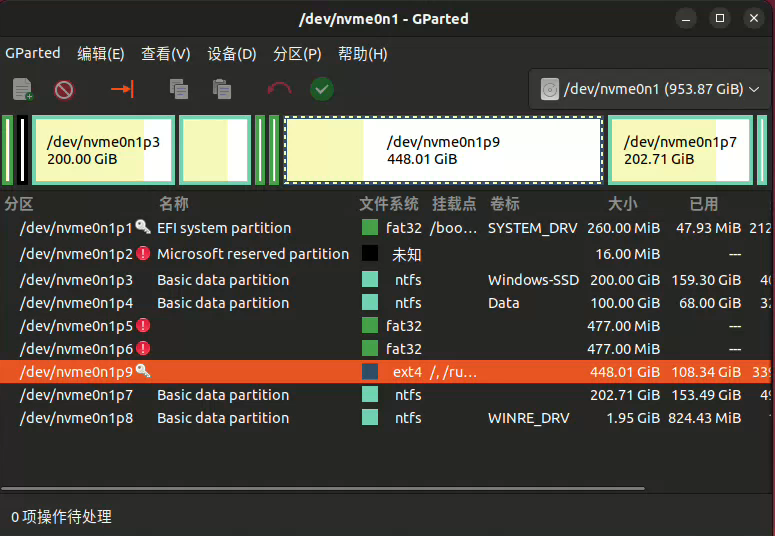
\includegraphics[width=0.85\textwidth]{linux10.png}
\caption{GParted}
\label{fig:linux10}
\end{figure}
\begin{figure}[H]
\centering
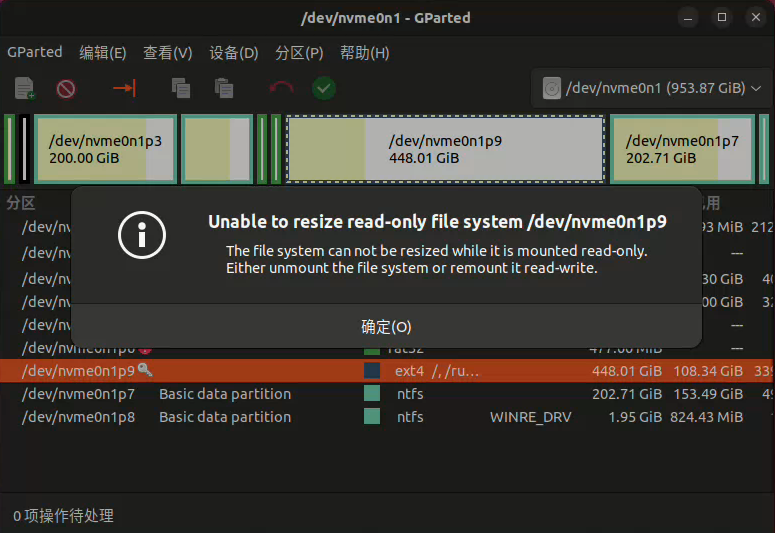
\includegraphics[width=0.85\textwidth]{linux9.png}
\caption{提示 “只读文件系统无法调整大小”}
\label{fig:linux9}
\end{figure}
但是如果这个时候你直接选择扩容，会发现有报错。为什么不能直接调整大小呢？因为当前 Ubuntu 的系统分区正在使用，通常要到另一个环境里才能移动。

这时候我们可以拿出安装时做好的启动盘，按之前的方法进入 Try Ubuntu。选择试用后，打开终端和 GParted，确认目标分区没有挂载，再按计划操作。扩容还需要合适位置的相邻未分配空间；如果中间隔着其他分区，就可能要移动它们，风险和耗时也会增加。\textbf{不要先在正在运行的系统里调节 swap 或其他分区位置}，担心的话先把完整计划交给学长核对，再到 Live 环境执行。

等待操作完成后重启，用 \texttt{lsblk} 和 \texttt{df -hT /} 分别核对分区容量与文件系统容量。它们看的不是同一层，只看一个数字变大还不够。具体限制可以查 \url{https://gparted.org/display-doc.php?name=help-manual}。
\begin{exercise}\label{ex:v1-resize-plan}
画出“根分区—其他分区—未分配空间”的布局，说明为何不能直接扩大根分区。写出备份、离线环境和结果核验计划。
\end{exercise}

\subsubsection{GRUB 美化*}
\label{sec:grub-theme}
也许你已经看腻了启动时那个黑框框，想把它换得好看一点。那我们接下来就给 GRUB 换个主题，不过先把两个系统都能启动这件事确认好，再来折腾外观。主题负责“长什么样”，默认进入哪个系统则要另外设置，装好主题不会顺手替你把这件事也做了。

下面展示的是 Tela 主题，对应项目在 \url{https://github.com/vinceliuice/grub2-themes}。在介绍 Git 之前，你可以先点击网页上的 Code → Download ZIP 下载。然后打开 README，按当前版本的说明选择主题名和分辨率参数；安装脚本也先读一遍，看看要改哪些文件，再决定是否执行。装其他主题的时候也要类似检查，别把来历不明的脚本直接交给 sudo，桌面颜值还没上去，启动先出问题就不划算了。
\Needspace{8\baselineskip}
\begin{example}[保存配置后检查默认项]
在 Ubuntu 中先保存原配置，再只读查看实际菜单标题：


\Needspace{7\baselineskip}
\begin{tbash}
sudo cp -a /etc/default/grub /etc/default/grub.before-training
grep '^GRUB_' /etc/default/grub
grep "^[[:space:]]*menuentry " /boot/grub/grub.cfg
\end{tbash}


如果你还希望没有操作时自动进入 Windows，我们就小小地配置一下引导。打开 \path|/etc/default/grub|，找到 \texttt{GRUB\_DEFAULT}，把它设为\textbf{本机实际菜单标题或稳定的菜单项 ID}。不过一般来说 Windows 是第三项。改完后运行 \texttt{sudo update-grub} 生成配置，确认没有报错；\texttt{grub.cfg} 是它生成出来的文件，别直接编辑。
\end{example}
\begin{note}
主题安装和引导配置改错可能妨碍选择启动项，所以记得保留可启动 U 盘和原配置。配置有误但 Ubuntu 仍能启动时，至少还可以按对应备份恢复并重新生成：


\Needspace{6\baselineskip}
\begin{tbash}
sudo cp -a /etc/default/grub.before-training /etc/default/grub
sudo update-grub
\end{tbash}

只有确认备份对应本次改动才恢复，别覆盖后来有意修改的配置。
\end{note}
\begin{figure}[H]
\centering
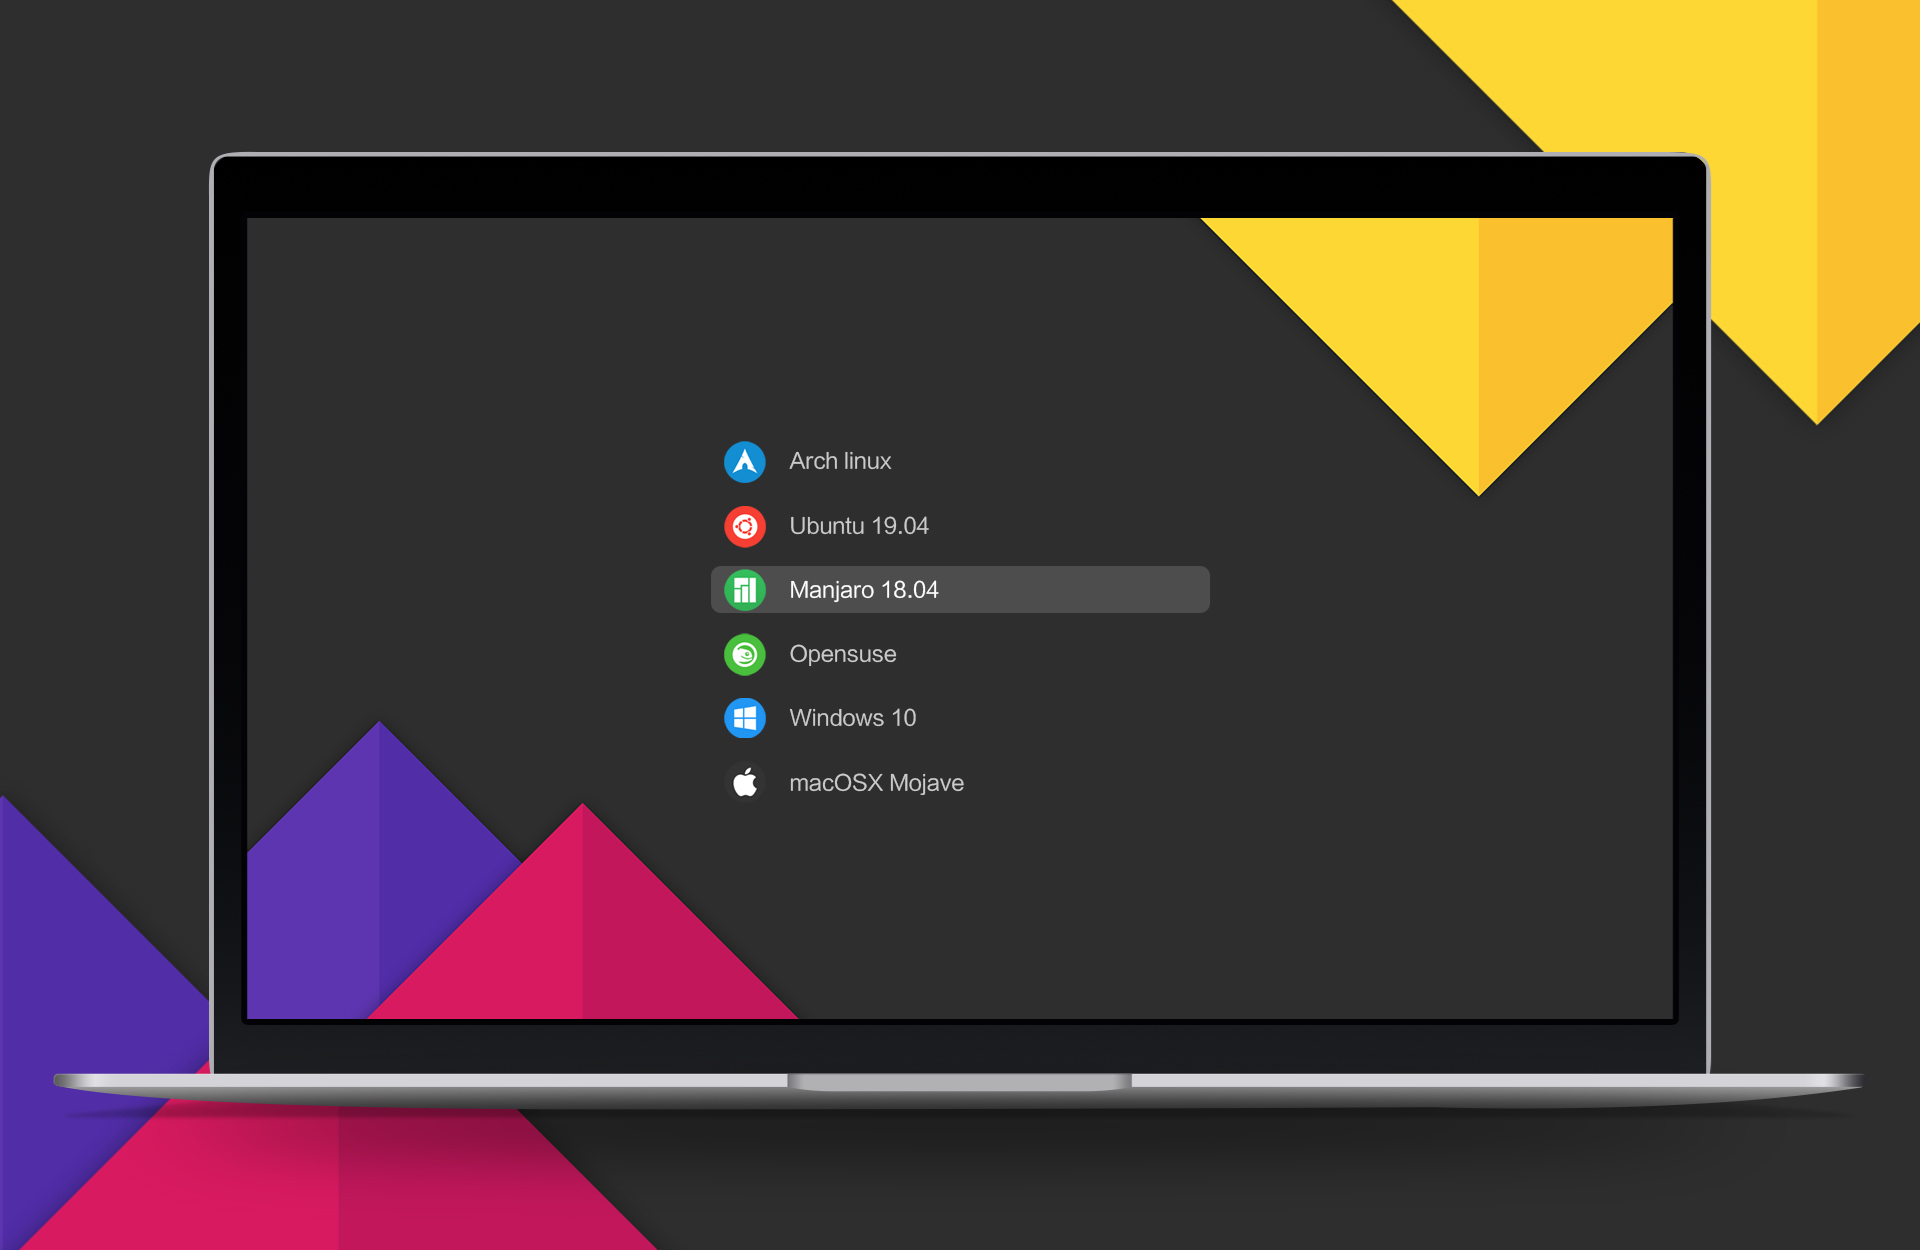
\includegraphics[width=0.8\textwidth]{grub.png}
\caption{Tela 主题效果示例}
\end{figure}

\subsubsection{桌面美化*}
\label{sec:gnome-customize}
GRUB 好看了，桌面也可以按自己的喜好收拾一下。Ubuntu 22.04 默认使用 GNOME，换个主题、装几个顺手的插件，就能让桌面更合你的习惯。

我们先分清要装的东西：主题主要改窗口外观，图标包改应用图标，Shell 扩展则增加桌面功能。它们各管一层，所以装了图标包，窗口颜色没变是正常的。先记下原来的外观，每次改一项，出了问题也更容易撤回。
\Needspace{8\baselineskip}
\begin{example}[主题的下载]
这里推荐一个美化网站 GNOME LOOK \url{https://www.gnome-look.org/browse/}，可以从这里挑选自己喜欢的主题(Gnome Shell Themes)或图标包(Full Icon Themes)下载，解压到用户目录。然后借助 Tweaks（优化）和Extension Manager（扩展管理器）进行美化的管理。下面的压缩包名要换成自己实际下载的文件名：


\Needspace{8\baselineskip}
\begin{tbash}
mkdir -p ~/.themes ~/.icons
tar -tf theme.tar.gz
tar -xf theme.tar.gz -C ~/.themes
sudo apt install gnome-tweaks gnome-shell-extension-manager
\end{tbash}


装好后打开 Tweaks， 在“外观”一栏选择刚装好的兼容主题或图标。有些 GTK4/libadwaita 应用不一定跟着 GTK3 主题改变，不用因为一个窗口没变色就把主题重装一遍。

接下来轮到 Extension Manager 了。打开“浏览”页，搜索你自己喜欢的扩展，点击安装。安装后在“已安装”页可以看到开关和设置按钮，开关控制启用状态，齿轮打开该扩展设置。注意有些扩展需要重启 GNOME 才能生效，可以按 Alt+F2 输入 r 回车重启。
\end{example}
\begin{figure}[H]
\centering
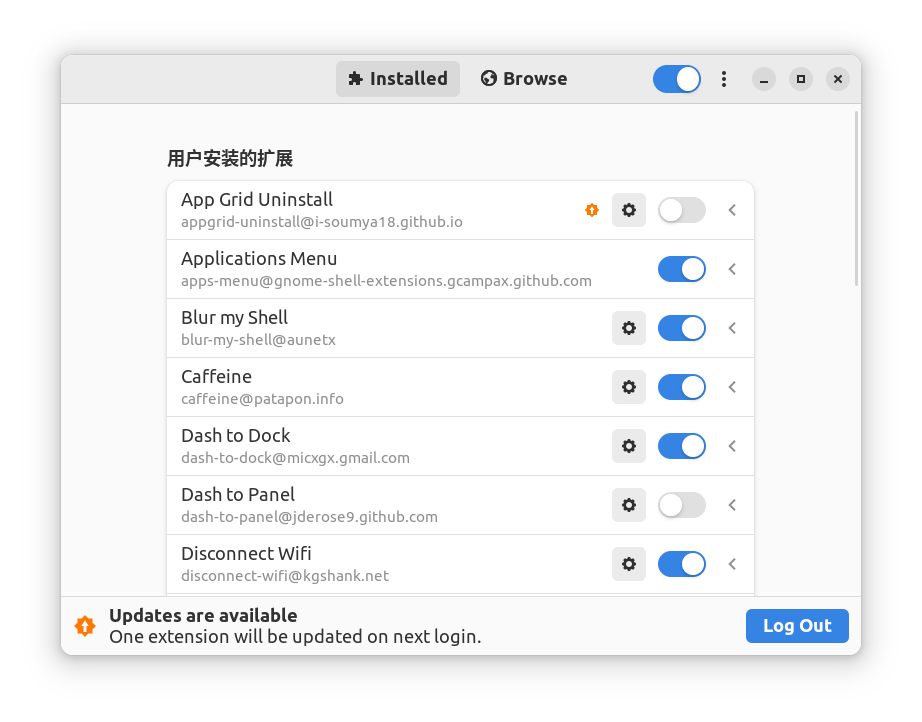
\includegraphics[width=0.8\textwidth]{gnome_extension_manager.png}
\caption{扩展管理器}
\label{fig:extension_manager}
\end{figure}
更多扩展可以在 \url{https://extensions.gnome.org/} 按版本查找。比如 Vitals 可以显示资源占用，Dash to Dock 可以调整程序坞，Clipboard Indicator 可以帮你找回刚刚复制过的文字, Caffeine让屏幕保持唤醒。建议先挑两三个顺手的，别一次全装——插件之间偶尔也会互相打架，尤其是 Dock 和 Panel 类扩展，装多了排查起来很痛苦。

\textbf{常用插件}

以下是视觉组往届同学常用的几款：

\begin{center}
\begin{tabular}{cc}
\toprule[1.5pt]
插件名 & 作用\\
\midrule[1pt]
Caffeine & 保持屏幕常亮，编译、跑数据集时防止自动锁屏\\
TopHat / Vitals & 在顶栏实时显示 CPU、内存、温度等信息\\
Dark Mode Toggle / Night Theme Switcher & 一键或按计划自动切换深色/浅色模式\\
Dash to Dock & 把左侧 Dock 栏变成可自定义的程序坞\\
Dash to Panel + ArcMenu & 合成类似 Windows 的底部任务栏与"开始菜单"\\
Rounded Window Corners Reborn & 给窗口加上圆角\\
Blur my Shell & 给顶栏、Dock 等加上毛玻璃半透明效果\\
Sound Input \& Output Device Chooser & 在右上角菜单直接切换声音输出/输入设备\\
Clipboard Indicator & 剪贴板历史记录，复制过的内容随时找回来\\
\bottomrule[1.5pt]
\end{tabular}
\end{center}

\begin{note}
上表插件的主页链接：

\begin{itemize}
\item Caffeine：\url{https://extensions.gnome.org/extension/517/caffeine/}
\item TopHat：\url{https://extensions.gnome.org/extension/5219/tophat/}
\item Vitals：\url{https://extensions.gnome.org/extension/1460/vitals/}
\item Night Theme Switcher：
\url{https://extensions.gnome.org/extension/2236/night-theme-switcher/}
\item Dash to Dock：\url{https://extensions.gnome.org/extension/307/dash-to-dock/}
\item Dash to Panel：\url{https://extensions.gnome.org/extension/1160/dash-to-panel/}
\item ArcMenu：\url{https://extensions.gnome.org/extension/3628/arcmenu/}
\item Rounded Window Corners Reborn：\par
\url{https://extensions.gnome.org/extension/7048/rounded-window-corners-reborn/}
\item Blur my Shell：\url{https://extensions.gnome.org/extension/3193/blur-my-shell/}
\item Sound Input \& Output Device Chooser：\par
\url{https://extensions.gnome.org/extension/906/sound-output-device-chooser/}
\item Clipboard Indicator：\url{https://extensions.gnome.org/extension/779/clipboard-indicator/}
\end{itemize}
\end{note}

\begin{figure}[H]
\centering
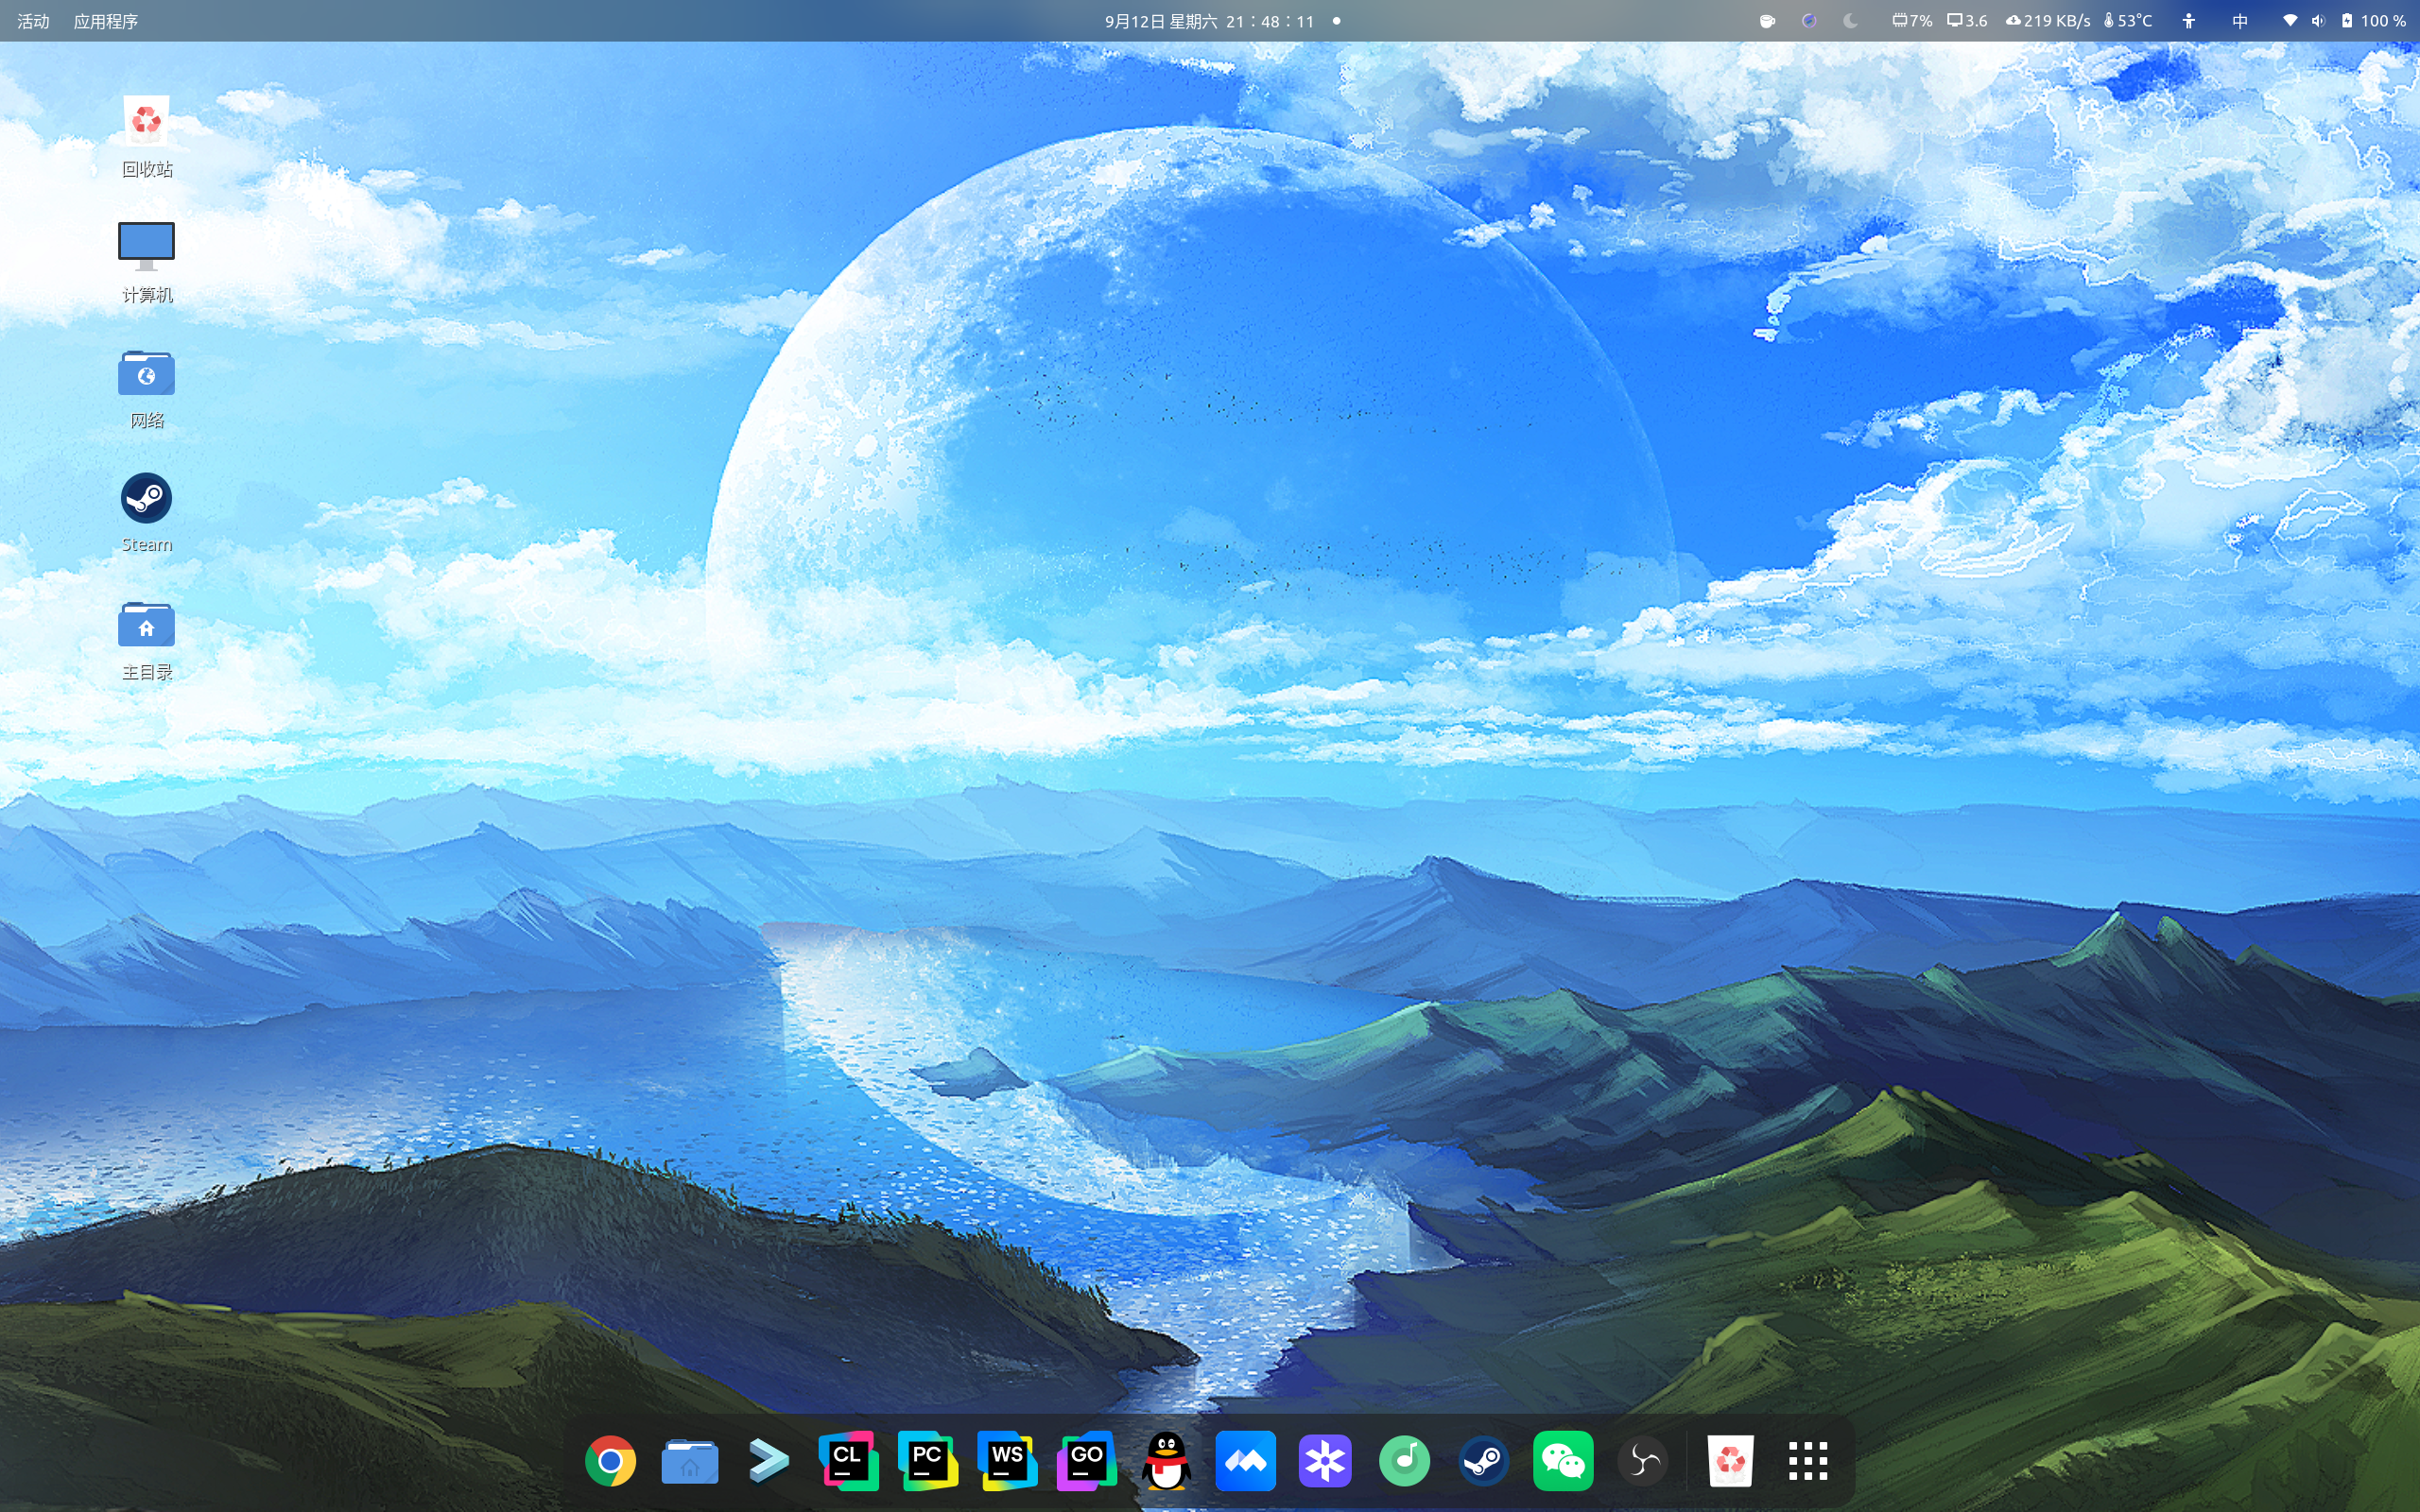
\includegraphics[width=0.85\textwidth]{gnome_desktop_after.png}
\caption{美化后的 GNOME 桌面}
\label{fig:desktop_after}
\end{figure}
